\setcounter{chapter}{1}
\chapter{Modèles de Drude et de Sommerfeld}
\section{Modèle de Drude}
\subsection{Modèle de Drude pour les métaux}
Malgré que le modèle de Drude soit ancien (1900) il est toujours utilisé 
aujourd'hui. A cette époque, l'électron n'a été mis en évidence que depuis 
trois ans : la physique quantique n'est pas encore connue mais les équations 
de Maxwell, elles, le sont bien.\\
Drude a voulu faire un \textit{modèle phénoménologique pour expliquer 
	les propriétés (conductivité électrique et thermique) des solides 
	(essentiellement les métaux).}\\
	
\noindent	
Au vu de la masse de la matière, Drude suppose qu'il existe des \textit{êtres 
lourds} (cœurs ioniques) autour desquels règne le vide permettant aux électrons 
de se déplacer.
	
\begin{wrapfigure}[11]{l}{7cm}
	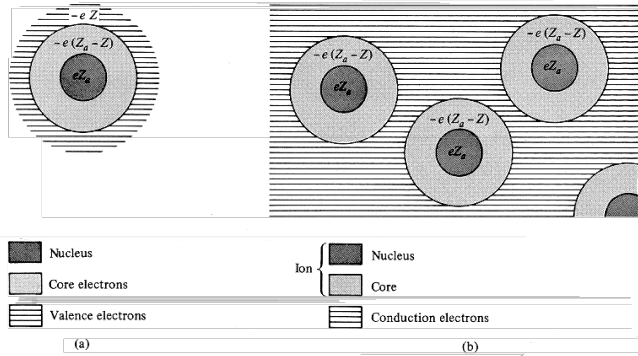
\includegraphics[scale=0.3]{ch1/image1.png}
	\captionof{figure}{Métal dans le modèle de Drude}
\end{wrapfigure}
\noindent
\textbf{	Inclure tableau slide}
Dans ce tableau, on peut voir $Z$ comme la valence, c'est à dire le nombre d'
électrons qui vont jouer dans le conduction\footnote{Ne pas confondre avec $Z_a$, 
le numéro atomique. On a donc $Z_a-Z$ électrons restant liés aux noyaux.}. La 
densité du gaz d'électron de valence, donnant le nombre d'électrons par volume, 
s'exprime 
\begin{equation}
	n = N_A * \dfrac{Z\rho_m}{A} \approx 10^{22}\ \frac{e^-}{cm^3}
\end{equation}
où $N_A$ est le nombre d’Avogadro, $\rho_m$ la masse spécifique du matériau 
([g/cm$^3$]) et $A$ la masse atomique de l'élément.
	
\noindent
Pour représenter cette densité, on utilise le paramètre $ r_s = \frac{r_0}{a_0}$
où $a_0$ est le rayon de Bohr \footnote{$a_0 = 4 \pi \epsilon_0 \frac{\hbar^2}{m_e e^2}$}
et $r_0$ le rayon d'une sphère contenant un seul 
électron. On a alors : 
\begin{equation}
	V_{sphère} = \frac{4\pi r^3_0}{3} = \text{Volume d'un électron} = \frac{1 e^-}{n} 
	\Longrightarrow r_0 = \left(\frac{3}{4\pi n}\right)^{1/3} \Longleftrightarrow r_s 
	= \left(\frac{3}{4\pi n a_0^3}\right)^{1/3}
\end{equation}
Ce paramètre est compris entre 2 et 3 pour la majorité des métaux et entre 3 et 6 
pour les métaux alcalins.
	
\newpage
\section{Hypothèses de base du modèle de Drude}
Pour parvenir à son modèle, Drude émit quatre hypothèses

\begin{enumerate}
	\item 
	      On postule l'\textit{
	      approximation des électrons indépendants} qui consiste à négliger l'interaction 
	      entre les électrons et l'\textit{approximations des électrons libre} qui consiste 
	      à négliger les interactions ion-électron. La première approximation est très
	      pertinente mais la deuxième est à abandonner pour une compréhension qualitative du
	      comportement des métaux. Ces approximations permettent de considérer que les électrons
	      suivent un mouvemment "classique" (MRU en l'absence de champ extérieur, etc...).
	      
	\item Collisions instantanées : la vitesse d'un électron change brusquement 
	      lors d'une collision avec un cœur ionique.
	      		
	\item C'est l'ingrédient phénoménologique : la probabilité de collision par unité de temps 
	      $1/\tau$ ([$s^{-1}$]) où $\tau$ est le temps de relaxation, que l'on suppose 
	      indépendant de la position et de la vitesse de l'électron\footnote{La probabilité 
	      	de subir une collision sur un intervalle de temps $dt$ est $dt/\tau$.}.
	      
	\item Les collisions amènent à un équilibre thermodynamque local
	      (après un nombre conséquent de collision, une seule ne suffit pas).
	      Immédiatement après une collision, l'électron a une direction aléatoire et une 
	      vitesse donnée par la distribution de la théorie cinétique des gaz.
\end{enumerate}


\section{Conductivité électrique "en courant continu" d'un métal}
On peut écrire la loi d'Ohm locale \footnote{ou bien $\vec(E) = \rho vec(j)$} 
\begin{equation}
	\vec{j} = \sigma\vec{E}
\end{equation}
où $\sigma$ est le conductivité électrique et $\vec{j}$ est le vecteur densité de 
courant, la densité de charge qui traverse une surface unitaire par unité de temps.\\

Soit $n$ électrons par unité de volume se déplaçant à vitesse moyenne $\vec{v}$. Sur 
$dt$, ils parcourent $vdt$ et donc $n(vdt)S$ électrons vont traverser une surface $S$ 
perpendiculaire au courant. La charge électrique traversant la surface sera $-envdtS$.
Comme $I = dQ/dt$, on a $I = -nevS$. Par définition, $J = I/S$. La densité de courant 
vaut alors
\begin{equation}
	\vec j = -e.n.S.\vec v\frac{1}{S} = -ne\vec{v}
\end{equation}

Le temps entre deux collisions est le temps de relaxation. Immédiatement après une collision 
la vitesse est $\vec{v_0}$. A cela nous rajoutons en plus la vitesse due à l'action du champ
sur la charge \footnote{$f = ma = eE \Leftrightarrow a = \frac{eE}{m} \Leftrightarrow
	v = \frac{eE\tau }{m}$} qui est $-e\vec{E}\tau/m$.
Par l'hypothèse 4, $\vec{v_0}$ ne contribue pas à la vitesse moyenne (pas de direction privilégiée) :
\begin{equation}
	\vec{v}_{moy} = \dfrac{-e\tau\vec E}{m}
\end{equation}
Avec la définition de $\vec j$, on obtient
\begin{equation}
	\vec j = \dfrac{ne^2\tau}{m}\vec{E}
\end{equation}
En en déduit avec la loi d'Ohm locale que\\
\

\retenir{
	\begin{equation}
		\sigma = \dfrac{ne^2\tau}{m}
	\end{equation}}

Le \textbf{tableau} donne des temps de relaxations $\tau$ calculés par Drude. A noter 
que son ordre de grandeur est $\approx\ 10^{-14}\ s$, ce que Drude avait conclut comme 
correct.  Hélas, la vitesse qu'il a considérée était fausse \footnote{Car la distribution 
des vitesses des électrons d'un métal n'est pas maxwellienne}. La vitesse exacte donne 
lieu à des distances moyennes entre deux collisions \footnote{calculées à partir de $\tau$
et $v_0$} plus grandes qui peuvent encore s’agrandir à basse température : l’hypothèse
des collision avec les cœur ionique est donc fausse, mais on peut utiliser  ce modèle
sans nous poser la question de la cause des collisions.

\section{Effet Hall et magnétorésistance}
Considérons un champ électrique $E_x$ selon $x$ appliqué au fil avec, en plus, un 
champ magnétique $\vec{H}$\footnote{C'est bien $\vec{H}$ le champ magnétique et non 
	$\vec B$ qui est la densité de champ d'induction magnétique ! Biot et Savart permet 
	en réalité de calculer $\vec{H}$ mais pas $\vec{B}$ (erreur fréquente). Cependant, 
	seul $\vec{B}$ est mesurable, $\vec{H}$ "n'existe pas".} dirigé selon $z$. La force 
de Lorentz exercée sur les $e^-$ vaut 
\begin{equation}
	-ev_x\vec{1_x}\times B\vec{1_z}
\end{equation}
Les électrons seront défléchis dans le sens $-y$ et un champ électrique $E_y$ va 
s'installer, dirigé vers les $y$ négatifs\footnote{Attention, la vitesse des 
	électrons est bien opposée à celle de $\vec{j}$}. Ce champ à l'équilibre va 
contrebalancer la force de Lorentz : $|E_y| = |v_x|B$.\\

Deux grandeurs sont remarquables :
\begin{enumerate}
	\item Remarquons la résistivité selon l'axe $x$ :
	      \begin{equation}
	      	\rho(B) = \dfrac{E_x}{j_x}
	      \end{equation}
	      C'est la \textit{magnétorésistance\footnote{La magnétorésistance est la propriété 
	      	qu'ont certains matériaux de présenter une résistance qui évolue lorsqu'ils sont 
	      soumis à un champ magnétique.} transverse} (car le champ magnétique est 
	      perpendiculaire au champ électrique), indépendante de $B$.
	      
	\item Le champ électrique transversal $E_y \propto B, j_x$. On définit le 
	      coefficient (ou constante) de Hall :
	      \begin{equation}
	      	R_H = \dfrac{E_y}{j_xB}
	      \end{equation}
\end{enumerate}

\begin{wrapfigure}[7]{l}{5.2cm}
	\vspace{-1cm}
	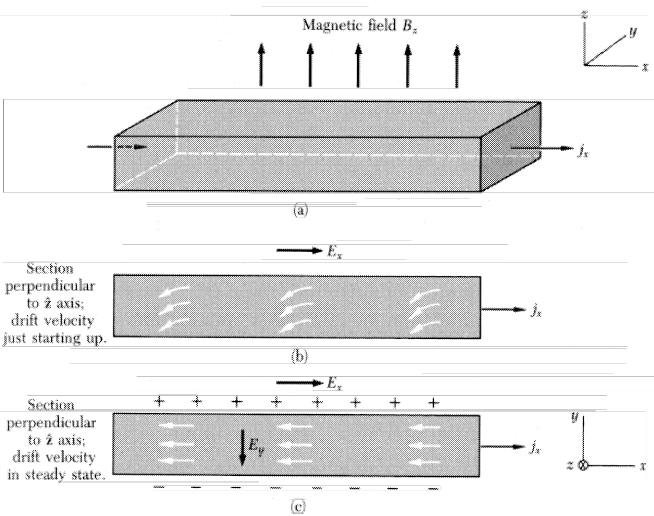
\includegraphics[scale=0.2]{ch1/image2.png}
	\captionof{figure}{Expérience de Hall}
\end{wrapfigure}
Le signe de $j_x$ est indépendant du signe des porteurs de charge ainsi que de la force
de Lorentz. Si les charges sont positives, $E_y$ et $R_H$ seront positifs. On peut 
calculer ce coefficient :
\begin{equation}
	-eE_y = ev_xB \Leftrightarrow -neE_y = nev_xB = j_xB \Longrightarrow R_H = -\frac{1}{ne}
\end{equation}
où $R_H$ est négatif car le champ de Hall est en -$\vec{1_y}$.



\newpage
\subsection{Conductivité thermique}
Le plus grand succès de ce modèle est d'avoir su expliquer la loi de 
Wiedemann-Franz disant que $\kappa/\sigma \propto \alpha T$ où $\alpha$ 
est une constante de proportionnalité. Dans son modèle, Drude suppose 
que la chaleur (courant thermique) est l'énergie cinétique des électrons
\footnote{Car les métaux conduisent mieux la chaleur.} (suivant une 
distribution de Maxwell).\\
Pour estimer $\kappa$, modélisons un barreau de cuivre avec des température 
élevé à gauche et faible à droite. Les électrons vont se déplacer plus ou 
moins rapidement, formant un gradient de température. 

\begin{equation}
	\vec{j}^Q = -\kappa\vec\nabla T
\end{equation}
Il s'agit de la loi de Fourier où $\kappa$ est la conductivité thermique. 
Pour calculer $\kappa$, faisons un bilan de courant de chaleur le tout 
un une dimension $x$ pour commencer, en considérant une surface transverse 
à notre belle barre.
\begin{itemize}
	\item[$\bullet$] La moitié des électrons vient de gauche, l'autre de droite.
	\item[$\bullet$] L'énergie thermique par un électron dans un métal à 
	      température d'équilibre $T$ est noté $\epsilon(T)$ (l'énergie cinétique 
	      dépend de la température).
	\item[$\bullet$] Si la dernière collision est en $x'$, sont énergie thermique 
	      est $\epsilon(T[x'])$.
	\item[$\bullet$] En moyenne, les électrons on subit leur dernière collision 
	      en $x - v\tau$ et ont une énergie de $\epsilon(T[x-v\tau])$.
\end{itemize}
On obtient alors
\begin{equation}
	j^Q = \frac{1}{2}nv[\epsilon(T[x-v\tau]) - \epsilon(T[x+v\tau])]
\end{equation}
La variation de température sur un $\ell pm$ étant faible, on peut développer 
$\vec{J}^Q$ en série autour de $x$\footnote{??} :
\begin{equation}
	j^Q = nv^2\tau\frac{d\epsilon}{dT}\left(-\dfrac{dT}{dx}\right)
\end{equation}
Drude suppose qu'après collision on a distribution des vitesses. Quand 
je passe en 3D, je prendrai comme vitesse moyenne $v_x^2 = \frac{1}{3}v^2$. 
Comme nous avons également
\begin{equation}
	n\frac{d\epsilon}{dT} = N/V\frac{d\epsilon}{dT} = \frac{dE/dT}{V} = c_v
\end{equation} 
où $c_v$ est la chaleur spécifique électronique par unité de volume. On 
a alors
\begin{equation}
	\vec{j}^Q = \frac{1}{3}v^2\tau c_v(-\vec{\nabla}T)
\end{equation}
Par identification avec la loi de Fourier 
\begin{equation}
	\kappa = \frac{1}{3}v^2 \tau c_v
\end{equation}
On peut obtenir le rapport suivant :
\begin{equation}
	\frac{\kappa}{\sigma} = \frac{1}{3}\frac{c_vmv^2}{ne^2}
\end{equation}
Comme on considère une distribution de Maxwell, la valeur de $c_v$ 
et de $<mv^2/2>$ sont connues (respectivement $(3/2)nk$ et $(3/2)k_BT$) :
\begin{equation}
	\frac{\kappa}{\sigma} = \frac{3}{2}\left(\frac{k}{e}\right)^2 T
\end{equation}
C'est la loi de Wiedemann-Franz. Le nombre de Lorentz $\kappa/\sigma T$ 
est bon\dots à un facteur 2 près. Ceci est du au fait qu'aucune 
contribution à la chaleur spécifique due aux électrons n'est observée et 
que $<v^2>$ et $c_v$ ne sont ici pas corrects.

\subsection{Modèle de Sommerfeld}
Il s'agit d'un modèle développé directement après l'avènement de la 
mécanique quantique. Il propose une première approche quantique des 
matériaux solides : des électrons dans une boîte. Ce modèle réglera 
le souci du facteur 2 et l'on pourra se passer de la contribution à 
la chaleur spécifique due aux électrons, fait non-observé 
expérimentalement.\\


Sommerfeld va supposer qu'un cristal solide peut être décrit par un 
puits fini, un cube de côté $L$.  En résolvant l'équation d'Erwin  
\begin{equation}
	\begin{array}{lll}
		                & H\psi                                            & =  \epsilon\psi      \\
		\Leftrightarrow & \left(-\frac{\hbar^2}{2m}\Delta + V_0\right)\psi & = \epsilon\psi       \\
		\Leftrightarrow & -\frac{\hbar^2}{2m}\Delta \psi                   & = (\epsilon+V_0)\psi 
	\end{array}
\end{equation}
Dont la solution est (notée sous la forme d'onde plane, plus 
intéressant)
\begin{equation}
	e^{i(k_xx-\omega t)}
\end{equation}
Ou seulement la partie spatiale :
\begin{equation}
	\Psi_k(\vec r) = \frac{1}{\sqrt{V}} e^{i\vec k \vec{r}}
\end{equation}
Si on remplace cette solution dans l'équation de Schrödinger\footnote{
Le gradient fait apparaître le $k^2$}, on obtient
\begin{equation}
	\frac{\hbar^2k^2}{2m} = (\epsilon-V_0)
\end{equation}
On va choisir des conditions aux limites qui sont un peu arbitraires :
il faudrait le faire via la conductivité électrique mais à l'époque ce 
n'est pas imaginable. L'état de surface d'un cristal n'est pas 
l'état en volume de ce cristal. Un électron est rarement influencé 
par l'état de surface, il ne va jamais très loin. On va introduire 
des CL arbitraire qui sont toujours utilisée : CI de Born-von Karman.\\

On ne veut pas que $\Psi(\vec{r})$ s'annule au bord car cela 
signifierait la présence d'un état stationnaire alors que le déplacement 
des électrons ne l'est pas (ondes progressives). On va alors imaginer 
un "cube" qui se refermerait sur lui même, c'est à dire que la fonction 
d'onde sur la face gauche du cristal est égal à la 
fonction d'onde sur la face opposée (droite en 1D) du cristal :
\begin{equation}
	e^{ik_xx} = e^{ik_x(x+L)}
\end{equation}
Cela introduit que 
\begin{equation}
	e^{ik_xL} = 1
\end{equation}
On en tire une équation de quantification imposant que
\begin{equation}
	k_x = \frac{2\pi}{L}n_x
\end{equation}
où $n_x$ est un nombre entier (qui n'est pas forcément le même 
que $n_y, n_z$). L'espace des vecteur $\vec{k}$ est un espace 
réciproque, c'est à dire un espace dual. Seuls les points dont les 
coordonnées sont des multiples entiers de $2\pi/L$ sont des vecteurs 
d'onde autorisés. Cela permet de connaître le nombre d'état possible 
dans une région de l'espace $\vec{k}$ plus grande que $2\pi/L$. 
Ces vecteurs $\vec k$ admis vont former un réseau de maille
$\frac{2\pi}{L}$ dans les direction $k_x,k_y$ et $k_z$.\\

Dans ces condition le nombres de points (états, vecteurs) autorisés 
est $\approx$ au volume de l'espace $\vec{k}$ divise par le volume 
de l'espace $\vec{k}$ contenant un seul point ($8\pi^3/V$).La densité 
de vecteur $\vec{k}$ autorisée dans l'espace réciproque vaut alors 
(l'inverse) 
\begin{equation}
	\frac{V}{8\pi^3}
\end{equation}

Les électrons sont des fermions : pour chaque vecteur $\vec k$ 
autorisé, il y a deux états électroniques possible (spin). Pour un 
grand nombre d'$e^-$, la région de l'espace $\vec{k}$ (réciproque) 
des états occupé est une sphère dont le rayon $k_F$, est le \textit{
	rayon de Fermi}. Son volume dans l'espace $\vec{k}$ vaut
\begin{equation}
	\sigma = \frac{4\pi}{3}k_F^3
\end{equation}
Le nombre de valeurs possibles de $\vec{k}$ dans cette sphère vaut 
\begin{equation}
	\left(\frac{4\pi k_F^3}{3}\right)\left(\frac{V}{8\pi^3}\right) = 
	\frac{k_F^3}{6\pi^2}V
\end{equation}
Il faut multiplier ce résultat par 2 pour tenir compte du spin.
\begin{equation}
	N = 2\frac{k_F^3}{6\pi^2}V = \frac{Vk_F^3}{3\pi^2}
\end{equation}
Si l'on a $N$ électrons dans un volume $V$, on obtient comme 
densité d'électron
\begin{equation}
	n = \frac{N}{V} = \frac{k_F^3}{3\pi^2}
\end{equation}
Cette sphère de rayon $k_F$ est la sphère de Fermi et son rayon est 
le nombre d'onde de Fermi. Sa surface est la "surface de Fermi" : 
elle sépare les états occupés des états vides.\\

On peut évaluer $k_F$ à partir du paramètre de densité électronique 
$r_s$ 
\begin{equation}
	\frac{3\pi^2}{k_F^3} = \frac{1}{n} = \frac{4\pi}{3}(r_sa_0)^3
\end{equation}
Le nombre d'onde de Fermi est de l'ordre de l'$\AA^{-1}$. La vitesse
de Fermi est donnée par $v_F = \hbar k_F/m$ et vaut $\approx 1000km/s$. 
Notons également que l'énergie de Fermi a un ordre de grandeur d'une 
dizaine d'eV.\\

En effectuant des calculs relativement simples mais laborieux, on 
peut obtenir l'expression de $c_v$ :
\begin{equation}
	c_v = \frac{\pi^2}{2}\left(\frac{k_BT}{\epsilon_F}\right)nk_B
\end{equation}

L'idée est maintenant de calculer la densité d'état en fonction de 
l'énergie en évaluant le nombre d'états électroniques compris entre 
deux sphères de rayon $k$ et $k'$. On va être amené à sommer les 
énergies sur tous les états.
\begin{equation}
	\sum_k = \alpha(k) \rightarrow \frac{V}{8\pi^3}\int\alpha(k)d\vec{k}
\end{equation}
Le nombre d'états étant important ($\approx 10^{22}$), on peut 
approximer cette somme par une majestueuse intégrale. Il y a un certain 
nombre d'états qui ont l'énergie recherchée dans la bande 
qui nous intéresse. En dérivant l'expression, on arrive à la densité 
d'état $\mathcal{D}(\epsilon)$.
\begin{equation}
	\mathcal{N}(\epsilon'+d\epsilon)
	-\mathcal{N}(\epsilon') \Longrightarrow \mathcal{D}(\epsilon) = 
	\frac{d\mathcal{N}(\epsilon)}{d\epsilon}
\end{equation}
où $\mathcal{N}(\epsilon)$ est le nombre d'états d'énergie $\leq 
\epsilon$. Cette énergie $\epsilon$ peut être obtenue via l'équation 
d'Erwin :
\begin{equation}
	\epsilon = \frac{\hbar^2k^2}{2m} + V_0 \Longrightarrow k = \sqrt{
		\frac{2m}{\hbar^2}(\epsilon-V_0)}
\end{equation}
En multipliant par un facteur deux pour tenir compte du spin, par la 
densité d'électron et le volume de la sphère de rayon $k$ on obtient 
le nombre d'électron $N(\epsilon)$.
\begin{equation}
	N(\epsilon) = 2 \frac{V}{8\pi^3}.\frac{4}{3}\pi k^3 = \frac{V}{3\pi^2}
	\frac{(2m)^{3/2}}{\hbar^3}(\epsilon-V)^{3/2}
\end{equation}
Si on dérive ça, on a la densité d'état par rapport à $\epsilon$ 
(attention : ne pas confondre $h$ et $\hbar$)
\begin{equation}
	\mathcal{D}(\epsilon) = \frac{d\mathcal{N}(\epsilon)}{d\epsilon}= 
	\frac{V}{2\pi^2}\frac{(Zm)^{(3/2)}}{\hbar^3}(\epsilon-V_0)^{1/2} = 
	\frac{4\pi V}{h^3} (2m)^{3/2)}(\epsilon-V_0)^{(1/2)}
\end{equation}

On peut arriver à une autre formulation en exprimant l'énergie en 
terme de $\epsilon/k_BT$\footnote{Il faudrait faire apparaître un 
facteur 2 pour tenir compte des deux états de spin.}. 
\begin{equation}
	\mathcal{D}(\epsilon)d\epsilon = \mathbb{N}V\frac{2}{\sqrt{\pi}}
	\left( \frac{\epsilon-V_0}{k_BT}\right)^{1/2}\frac{d\epsilon}{k_BT}
\end{equation}
où $\mathbb{N}$ est la densité effective d'états
\begin{equation}
	\mathbb{N} = \frac{2}{h^3}(2\pi m k_BT)^{3/2}
\end{equation}
Pour la température $T$, le nombre d'électrons ayant des énergies 
comprises entre $\epsilon$ et $\epsilon+d\epsilon$ vaut 
\begin{equation}
	\mathcal{D}(\epsilon)f(\epsilon)d\epsilon
\end{equation}
où $f(\epsilon)$ exprime la probabilité d'occupation d'un état 
d'énergie $\epsilon$ grâce à la distribution de Fermi-Dirac.\\

Comment va-t-on faire à température nulle? On peut dire que 
$\mu = \epsilon_f$ en se basant sur cette même distribution. En 
effet, comme $T\rightarrow 0$, il faut nécessairement que $\epsilon
= \mu$ sans quoi un souci se poserait. La concentation d'électron 
vaut alors
\begin{equation}
	n = \int_{V_0}^\infty \mathcal{D}(\epsilon)d\epsilon = 
	\int_{V_0}^{\epsilon_F=\mu}\mathcal{D}(\epsilon)d\epsilon 
\end{equation}
A température non-nulle, il suffit de considérer l'infini comme borne 
supérieure sans oublier de faire apparaître la distribution de FD.
\begin{equation}
	n = \int_{V_0}^\infty \mathcal{D}(\epsilon)f(\epsilon)d\epsilon
\end{equation}
En explicitant
\begin{equation}
	n = \mathbb{N}\frac{2}{\sqrt{\pi}}\int_{V_0}^\infty \frac{1}{e^{
		(\epsilon-V_0)/k_BT}+1}\left(\frac{\epsilon-V_0}{k_BT}\right)^{1/2
	}\frac{d\epsilon}{k_BT}
\end{equation}
Le changement de variable
\begin{equation}
	\eta = \frac{\epsilon - V_0}{k_BT}
\end{equation}
nous donne
\begin{equation}
	\frac{n}{\mathbb{N}} = \frac{2}{\sqrt{\pi}}\int_0^\infty \dfrac{\sqrt
		{\eta}}{e^{(\eta-\zeta)/k_BT}+1}d\eta
\end{equation}
où $\zeta(n/\mathbb{N}) = \mu - V_0$, dont l'ordre de grandeur typique 
est 
d'une dizaine d'électron volt.\\
Voyons comment $\zeta$ dépend de $n/\mathbb{N}$.
\begin{enumerate}
	\item $\zeta$ fortement négatif (cas non-dégénéré)\\
	      L'exponentielle du dénominateur est grande devant 1. En première 
	      approximation, cela donne :
	      \begin{equation}
	      	\frac{n}{\mathbb{N}} \approx \frac{2}{\sqrt{\pi}}\int_0^\infty e^{-
	      		\eta + \frac{\zeta}{k_BT}}\sqrt{\eta}d\eta = \frac{2}{\sqrt{\pi}}
	      	\underbrace{\int_0^\infty e^{-\eta} \sqrt{\eta}d\eta}_{\Gamma(\frac{3
	      		}{2}) = \frac{1}{2}\Gamma(\frac{1}{2}) = \frac{1}{2}\sqrt{\pi}}.e^{
	      	\zeta/k_BT} = e^{\zeta/k_BT}
	      \end{equation}
	      Ce cas s'applique aux semi-conducteurs ($n/\mathbb{N}\ll 1$). On en 
	      déduit que
	      \begin{equation}
	      	\zeta = k_BT\ln\frac{n}{\mathbb{N}}
	      \end{equation}
	\item $\zeta$ fortement positif (cas dégénéré)\\
	      L'exponentielle du dénominateur est petite devant 1 et ce tant que $
	      \eta < \zeta/k_BT$. On approxime en remplaçant l'intégrande par 1 dans 
	      un intervalle réduit (de 0 à $\zeta/k_BT$) :
	      \begin{equation}
	      	\frac{n}{\mathbb{N}} \approx \frac{2}{\sqrt{\pi}}\int_0^{\zeta/k_BT} 
	      	\sqrt{\eta}d\eta = \frac{4}{3\sqrt{\pi}}\left(\frac{\zeta}{k_BT}\right)^{
	      	3/2}
	      \end{equation}
	      et nous en déduisons cette fois-ci que $1 \ll \frac{n}{\mathbb{N}}$. On 
	      retrouve ceci dans les métaux.
\end{enumerate}
Notons que dans la plupart des semi conducteurs, on a un $\zeta$ négatif du 
aux impuretés que l'ont doit ajouter pour venir peupler la bande de valence.



\subsection{Condition générale d'équilibre thermique}
On modélise deux solides différent par le modèle Sommerfeld, c'est-à-dire 
deux profondeurs de puits différents. On va remplir tous les puits (niveaux 
d'énergie) jusqu'à une énergie maximale. Il faudrait un miracle pour avoir 
le même niveau d'énergie dans les deux métaux. On imagine que les électron 
$A$ vont voir des espaces libre à plus basse énergie dans $B$ et vont y aller. 
Si on a par ex un manque d'électron en $A$ et un excès en $B$ on va avoir un 
champ électrique, créant un potentiel de contact et égalant les niveaux de 
Fermi. La condition d'équilibre est que le niveau d'énergie de Fermi soit le 
même dans tous l'espace. \textit{"Je détaille pas trop ici."} 

\begin{center}
	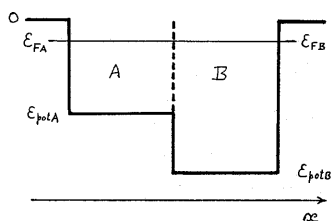
\includegraphics[scale=0.6]{ch1/image3.png}
	\captionof{figure}{Condition générale d'équilibre thermique}
\end{center}
